%!TEX encoding = UTF-8 Unicode
% !TeX spellcheck = en_GB
%%%%%%%%%%%%%%%%%%%%%%%%%%%%%%%%%%%%%%
\chapter{ Virtual two-loop calculation of  $Zh$ production via gluon fusion}\label{chap:hz}
%%%%%%%%%%%%%%%%%%%%%%%%%%%%%%%%%%%%%%
\par As we have seen in~\autoref{sec:Higgscoupl}, Higgs couplings to the weak vector bosons, i.e. $Z$ and $W$ is approaching the precision level. For their measurements both VBF and $Vh$ channels are used, the associated Higgs production with the vector bosons are not only important for measuring the $VVh$ coupling but also other couplings and properties as discussed in~\autoref{vhproduction}. The most notable example emphasising the importance of this channel is the measurement of the Higgs decaying to beauty quarks~$h \rightarrow b \bar{b}$ by both ATLAS and CMS~\cite{Aaboud:2018zhk, Sirunyan:2018kst}. Hence, the~$Vh$ Higgs production is an important channel to look for in the future runs of the LHC. As the statistical and systematic uncertainties coming from the experimental setup of the LHC will be eventually reduced in the future runs, due to higher integrated luminosity,  upgraded detectors and improved analysis techniques. There is an exigency to reduce theoretical uncertainties emerging from the perturbative calculations of  cross-sections. In order to accomplish that, one should include higher order terms to the theoretical prediction. Since $Wh$ production has no gluon fusion channel, and the main source of $Zh$ uncertainties actually come from its gluon fusion part. Higher order correction to the $gg \to Zh$ is the key to improve the theoretical modelling for $Vh$. \\ 
It should be noted that the $Zh$ channel can receive contributions from new particles \cite{Harlander:2013mla}, particularly at the large invariant-mass region where the gluon fusion contribution becomes more important, and HTL approximation would typically fail. Therefore, better understanding of the SM prediction of the $Zh$ gluon fusion channel is crucial for both the SM precision measurements of Higgs production within the SM and for testing NP in this channel, e.g. new vector-like leptons.  \\ This chapter aims to demonstrate the use of $\pt$--expansion technique, developed in ~\cite{Bonciani:2018omm} as an approach to compute the two-loop virtual corrections to $gg \to Zh$ analytically, including top mass effects. This method also allows for the use of  Pad\'e approximants, in order to extend the range of validity of this calculation.\la{cite the paper once it is out}
\par This chapter is structured as follows : In~\autoref{chap6sec:GenNot} contains the general notation we have used for the gluon fusion $Zh$ process calculation. Then, in~\autoref{sec:ptexp} the transverse momentum expansion method is discussed.  Calculation of the LO form-factors in the transverse momentum expansion is illustrated in~\autoref{sec:LOPtExp} as a proof of concept for the $\pt$-expansion technique. Outline of the two-loop calculation is discussed in~\autoref{sec:quattro}. Finally, in~\autoref{sec:hzres}, the results of our calculation are shown with concluding remarks at the end.  This chapter is based on the work my collaborators and I have published in ~\cite{Alasfar:2021ppe}. 
%%%%%%%%%%%%%%%%%%%%%%%%%%%%%%%%%%%%%%%%%%%%%%%%%
\section{General notation \label{chap6sec:GenNot} }
\par The amplitude  $g^\mu_a(p_1)g^\nu_b(p_2)\to Z^\rho(p_3) h(p_4)$ can be written as
\begin{align}
&&\amp=i \sqrt{2}\frac{\mz \Gfer \as(\mu_R)}{\pi}\delta_{ab}\epsilon^a_\mu(p_1)
\epsilon^b_\nu(p_2)\epsilon_\rho(p_3)\hat{\amp}^{\mu\nu\rho}(p_1,p_2,p_3 ),\\
&&\hat{\amp}^{\mu\nu\rho}(p_1,p_2,p_3 )=\sum_{i=1}^{6}
\mathcal{P}_i^{\mu\nu\rho}(p_1,p_2,p_3 )
\amp_i(\hat{s},\hat{t},\hat{u},\mt,\mh,\mz),
\label{eq:amp}
\end{align}
where  $\mu_R$ is the renormalisation scale and
$\epsilon^a_\mu(p_1)\epsilon^b_\nu(p_2)\epsilon_\rho(p_3)$ are the
polarization vectors of the gluons and the $Z$ boson, respectively.  It is possible to decompose the amplitude into a maximum of $6$ Lorentz structures encapsulated by the 
tensors $\mathcal{P}_i^{\mu\nu\rho}$. Due to the presence of the~$\gamma_5$ these projectors are
proportional to the Levi-Civita total anti-symmetric tensor
$\epsilon^{\alpha\beta\gamma\delta}$. One can choose to an orthogonal basis explicitly shown in~\autoref{app:uno}, such that
\begin{equation}
	\mathcal{P}_i^{\mu\nu\rho} \mathcal{P}_j\,_{\mu\nu\rho} = 0, \,\,\, \,\, \text{for}\, i \neq j 
\end{equation}
By this choice one obtains unique form factors corresponding to each projector
\begin{equation}
\amp_i(\hat{s},\hat{t},\hat{u},\mt,\mh,\mz),
\end{equation}
 that are multivariate complex functions of the
top ($\mt$), Higgs ($\mh$) and $Z$ ($\mz$) bosons masses, and of
the partonic Mandelstam variables
\begin{equation}
\hat{s}=(p_1+p_2)^2,~~ \hat{t}=(p_1+p_3)^2,~~ \hat{u}=(p_2+p_3)^2,
\end{equation}
where $\hat{s}+\hat{t}+\hat{u}=\mz^2+\mh^2$ and all the momenta are considered to
be incoming. 
The form-factors~ $\amp_i$ can be perturbatively expanded in orders of~$\alpha_s$, 
\begin{equation}
\amp_{i} = \sum_{k=0} \left(\frac{\alpha_s}{\pi} \right) ^k \amp_i^{(k)}
\label{eq:ampexp}
\end{equation}
Where~$\amp_i^{(0)}$ and $\amp_i^{(1)}$ are the LO and NLO terms, respectively. Using Fermi's Golden Rule, we can write thee Born partonic cross-section as
\begin{equation}
\hat{\sigma}^{(0)}(\hat{s})=
\frac{\mz^2 \Gfer^2 \alpha_s(\mu_R)^2}{64 \hat{s}^2(2\pi)^3}
\int^{\hat{t}^+}_{\hat{t}^-}d\hat{t}\sum_i \left|\amp_i^{(0)}\right|^2,
\end{equation}
where
$\hat{t}^\pm=[-\hat{s}+\mh^2+\mz^2\pm\sqrt{(\hat{s}-\mh^2-\mz^2)^2-4\mh^2\mz^2}\,]/2$.
\begin{figure}
	\begin{center}
		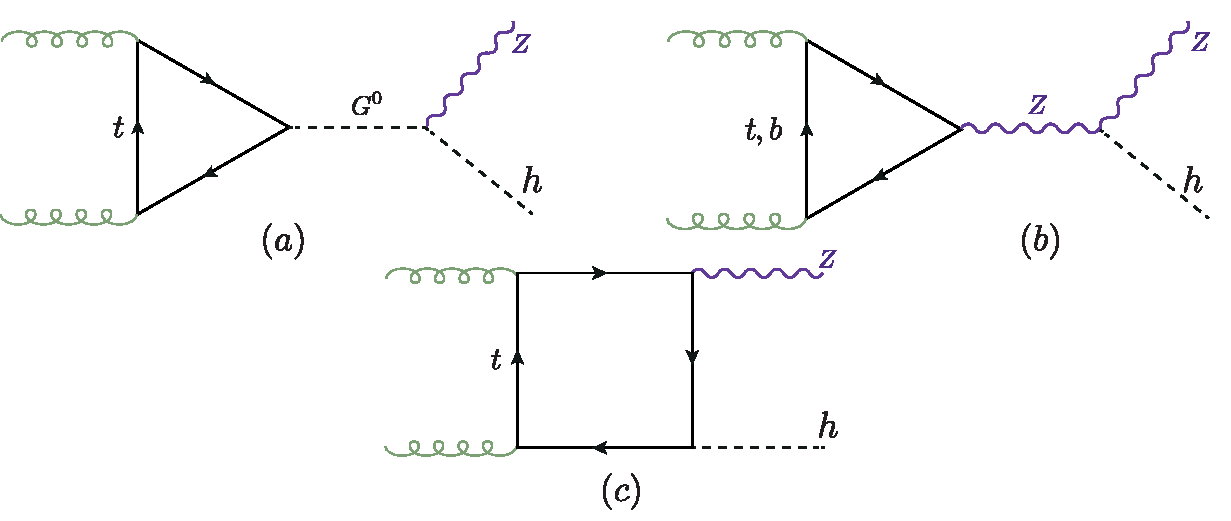
\includegraphics[width=12cm]{./figures/Feynman_LO}
		\caption{Feynman diagrams type for the LO $gg \to Zh$ process. The triangle diagrams in a general $\xi$ gauge involve $Z$ and the neutral Goldstone~$G^0$ propagators. }
		\label{fig:dialo}
	\end{center}
\end{figure}
\par The LO has two sets of diagrams, the triangle, and box diagrams shown in~\autoref{fig:dialo}. In (a), the triangle diagrams contains a neutral Goldstone boson~$G^0$, instead in (b) the $Z$ boson is mediated. The interplay between these two diagram types depends on the~$\xi$ gauge. Moreover, the $Z$ boson is strictly off-shell, due to Furry's theorem.
In the Landau gauge the $Z$- mediated diagrams will also vanish, this can be seen by considering the subamplitude~$ggZ^*$ which in the Landau gauge can be related to the decay of a massive vector boson
with mass $\sqrt{\hat{s}}$ into two massless ones, a process that is
forbidden by the Landau-Yang theorem \cite{Landau:1948kw,Yang:1950rg}.
The triangle diagrams are also proportional to the mass difference between the up and down type quarks. In this calculation, the first and second generation quarks are assumed to be massless, as well as the $b$ quark, hence light quarks loops  do not contribute to this process. The same would apply to the box diagrams (c), as they are proportional to the quark Yukawa coupling, and vanish in the massless quarks case. Moreover, triangle diagrams with $b-$ quark loops contribute to $ \sim 1\%$ of the total amplitude, computed in the limit $m_b \to 0$.  
%%%%%%%
\subsection{The transverse momentum expansion}
\label{sec:ptexp}
\par Choosing to expand in small $\pt$ of the $Z$ boson, the first step is expressing $\pt$ in terms of the Mandelstam variables and masses 
\beq
\pt^2=\frac{\hat{t}\hat{u}-\mz^2\mh^2}{\hat{s}}.
\label{ptdef}
\eeq
From  eq.(\ref{ptdef}), together with the relation between
the Mandelstam variables, one finds 
\beq
\pt^2+\frac{\mh^2+\mz^2}{2}\leq\frac{\hat{s}}{4}+\frac{\dm^2}{\hat{s}},
\label{ptexp}
\eeq
where
$\dm = (\mh^2 -\mz^2)/2$. Eq.(\ref{ptexp}) implies 
$\pt^2/\hat{s} < 1$ that, together with the kinematical constraints
$\mh^2/\hat{s}< 1$ and
$\mz^2/\hat{s} < 1$. With these relations in mind, one can expand the amplitudes in terms of small  $\pt^2/\hat s$, $\mh^2/\hat{s}$ and $\mz^2/\hat{s}$, which is technically valid throughout the whole phase space, contrary to the LME and HE limits.  The caveat for this expansion is that, the amplitude does not depend on $\pt$ explicitly. Instead, one would expand in the reduced Mandelstam variables~$t^\prime/s^\prime\ll 1$ or $u^\prime/s^\prime\ll 1$, defined as
\beq
s^\prime=p_1\cdot p_2=\frac{\hat{s}}{2},~~
t^\prime=p_1\cdot p_3=\frac{\hat{t}-\mz^2}{2},~~ u^\prime =
p_2\cdot p_3=\frac{\hat{u}-\mz^2}{2}
\eeq
and satisfy
\beq
s^\prime + t^\prime + u^\prime =\dm.
\eeq
The choice of the expansion parameter~$t^\prime$ or ~$u^\prime$  depends whether one expands in the forward or backwards kinematics. Because the process $gg \to Zh$, has two particles in the final states with different masses, the amplitude is not symmetric under the their exchange. One therefore cannot compute the cross-section by integrating only the forward-expanded amplitude~\cite{Alasfar:2021ppe}, contrary what has been done for the Higgs pair~\cite{Bonciani:2018omm}. In order to overcome this issue, one could further examine the projectors in~\autoref{app:uno} and observe that they can be split into symmetric and anti-symmetric parts with respect to the exchange $ t^\prime \leftrightarrow u^\prime$. Then, expand the symmetric part in the forward kinematics, like the Higgs pair case. As for the anti-symmetric part, the antisymmetric factor is simply extracted by multiplying the form-factors by $1/(\hat{t}-\hat{u})$,
written as $1/( 2 s^\prime - 4 t^\prime - 2 \dm)$, then perform the expansion in the forward kinematics and finally multiply back by $(\hat{t}-\hat{u})$.

\par In order to implement the $\pt$-expansion at the Feynman diagrams level we start by splitting the momenta into longitudinal and transverse with respect to the beam direction, by introducing the vector~\cite{Bonciani:2018omm}, 
\begin{align}
r^\mu &= p_1^\mu +p_3^\mu,
\end{align}
 which satisfies
\beq
r^2= \hat{t},~~ r\cdot p_1=\frac{\hat{t}-\mz^2}{2},~~
r\cdot p_2=-\frac{\hat{t}-\mh^2}{2},
\label{rsp}
\eeq
and hence can be also written as
\beq
r^\mu =-\frac{\hat{t}-\mh^2}{\hat{s}}p_1^\mu +
\frac{\hat{t}-\mz^2}{\hat{s}} p_2^\mu + r_\perp^\mu =
\frac{t^\prime}{s^\prime}\,(p_2^\mu -p_1^\mu) - \frac{\dm}{s^\prime} \, p_1^\mu +
r_\perp^\mu,
\label{rpp}
\eeq
where
\beq
r_\perp^2=-\pt^2.
\eeq
substituting the definition of~$\pt$ from eq.\eqref{ptdef} one obtains
\beq
t^\prime = -\frac{s^\prime}2 \left\{ 1 - \frac{\dm}{s^\prime} \pm
\sqrt{\left( 1 - \frac{\dm}{s^\prime} \right)^2 -
	2 \frac{\pt^2 + \mz^2}{s^\prime}} \right\}
\label{tpdef}
\eeq
implying  that the expansion in
small $\pt$ (the minus sign case in eq.(\ref{tpdef})) can be realized
at the level of Feynman diagrams, by expanding the propagators
in terms of the vector $r^\mu$ around $r^\mu \sim 0$ or, equivalently,
$p_3^\mu \sim -p_1^\mu$, see eq.(\ref{rpp}). 

\section{Born cross-section in the $\pt$-expansion }
\label{sec:LOPtExp}
\par As a baseline test for the validity and convergence behaviour of the~$\pt$ expansion we start by computing the LO amplitude, and consequently the Born partonic cross-section in the $\pt$ expansion then compare it with the exact results found in~\cite{Kniehl:1990iva, Dicus:1988yh} . \\ Starting by defining the one-loop functions appearing in the similar calculation of the Born cross-section for ~$gg \to hh$ in the same expansion carried out in ref.~\cite{Bonciani:2018omm}
\bea
B_0[\hat{s},\mt^2,\mt^2] \equiv  B_0^+, &
B_0[- \hat{s},\mt^2,\mt^2]  \equiv B_0^- , &\\
C_0[0,0,\hat{s},\mt^2,\mt^2,\mt^2]  \equiv  C_0^+  ,& ~~~
C_0[0,0,-\hat{s},\mt^2,\mt^2,\mt^2]  \equiv C_0^- &
\eea
\beq
B_0[q^2,m_1^2,m_2^2] = \frac1{i\pi^2}
\int \frac{d^n k}{\mu^{n-4}} \frac1{(k^2 -m_1^2)((k+q)^2-m_2^2)},
\label{Bzero}
\eeq
\begin{align}
	%	\specialcell
	{ C_0[q_a^2,q_b^2,(q_a+q_b)^2, m_1^2,m_2^2,m_3^2] = \hfill }\nn  \\
	\frac1{i\pi^2}  \int \frac{d^d k}{\mu^{d-4}} \frac1{[k^2 -m_1^2][(k+q_a)^2-m_2^2]
		[(k-q_b)^2 - m_3^2]} &
	\label{Czero}
\end{align}
are the Passarino-Veltman functions \cite{Passarino:1978jh},
with $d$ the dimension of spacetime and $\mu$ the 't Hooft mass.
%
There are only two non-vanishing form-factors at LO, one is symmetric~${\cal A}_2$, and the other is antisymmetric~${\cal A}_6$, in the $\pt$-expansion, these form-factors are give by, up to order ~${\mathcal O}(\pt^2)$
\bea
\mathcal{A}_{2}^{(0, \triangle)} &=& -
\frac{ \pt }{\sqrt{2} \left( \mz^2+\pt^2 \right)} (\hat{s}-\dm)\,
\mt^2 C_0^+,
\label{Adt}\\
\mathcal{A}_{2}^{(0, \square)} &=&
\frac{ \pt }{\sqrt{2} \left(\mz^2+\pt^2 \right)}\, \Biggl\{ \Biggr. \nn \\
&& \Biggl( \mt^2 -\mz^2 \frac{ \hat{s}-6 \mt^2}{4 \hat{s}}-
\pt^2 \frac{ 12 \mt^4-16 \mt^2 \hat{s}+\hat{s}^2}{12 \hat{s}^2}
\Biggr)  B_0^+ \nn \\
&-& \Biggl( \mt^2 -\dm  \frac{\mt^2}{ \left( 4 \mt^2+\hat{s}\right)}
+ \mz^2 \frac{ 24 \mt^4 -6 \mt^2 \hat{s}-
	\hat{s}^2 }{4 \hat{s} \left(4 \mt^2+\hat{s}\right)} -
\nn \\
& & ~~~~~~~\pt^2 \frac{ 48 \mt^6-68 \mt^4 \hat{s}-4
	\mt^2 \hat{s}^2+\hat{s}^3 }{ 12 \hat{s}^2 \left(
	4 \mt^2 +\hat{s} \right) }  \Biggr)
B_0^- \nn \\
&+&\Biggl( 2 \mt^2- \dm +
\mz^2 \frac{3 \mt^2-\hat{s}}{\hat{s} } +
\pt^2  \frac{ 3 \mt^2 \hat{s}-2 \mt^4 }{\hat{s}^2}\Biggr)
\mt^2 \, C_0^- \nn \\
& +&\Biggl( \hat{s}-2 \mt^2 +
\mz^2  \frac{\hat{s}-3 \mt^2 }{\hat{s}}+
\pt^2 \frac{ 2 \mt^4-3 \mt^2 \hat{s}+\hat{s}^2}{\hat{s}^2 }\Biggr)
\mt^2 \, C_0^+ \nn \\
& +&\log \left(\frac{\mt^2}{\mu^2}\right) \frac{ \mt^2}{\left(4
	\mt^2+\hat{s}\right) } \Biggl( \dm + 2  \mz^2
+\pt^2 \frac{2   \hat{s}-2 \mt^2}{3 \hat{s} }\Biggr)\nn  \\
&-&\dm \frac{2 \mt^2}{\left(4 \mt^2+\hat{s}\right) } +
\mz^2  \frac{\hat{s}-12 \mt^2}{4 \left(4 \mt^2+\hat{s}\right)}
+\pt^2 \frac{ 8 \mt^4-2 \mt^2 \hat{s}+ \hat{s}^2 }
{4\hat{s} ( 4\mt^2 + \hat{s})}  \Biggl. \Biggl\},\nn \\
&&
\label{Adb}
\eea
and
\bea
\mathcal{A}_{6}^{(0, \triangle)} &=&  0,
\label{Ast} \\
\mathcal{A}_{6}^{(0, \square)} &= & 
\frac{\hat{t}-\hat{u}}{\hat{s}^2} \,\pt \Biggl[ \frac{\mt^2}2
\Bigl( B_0^- - B_0^+ \Bigr) -\frac{\hat{s}}{4} \nn \\
& -&\frac{2 \mt^2+\hat{s}}{2}\mt^2 \, C_0^- 
+\frac{2 \mt^2-\hat{s}}{2} \mt^2 \,C_0^+  \Biggr],
\label{Asb}
\eea
where these form-factors were divided into triangle ($\triangle$) and
box ($\square$) contributions, and $B_0$ functions are understood as the
finite part of the integrals on the right hand side of eq.\eqref{Bzero}.
\par Using several truncations of the $\pt$-expansion, and comparing it to the exact LO result, one can see in~\autoref{fig:LO} the exact Born partonic LO cross section (red line) as a function of the invariant mass of the $Zj$ system, $M_{Zh}$, in comparison to the $\pt$-expansions. 
For the numerical evaluation of the cross section here and in
the following, we used as SM input parameters
\begin{equation}
	\begin{split}
		\mz=91.1876 \,\gev, ~~\mh=125.1 \gev, ~~  \mt=173.21\, \gev, \nn\\
		m_b = 0 \, \gev, ~~G_F= 1.16637\,\gev^{-2},~~ \alpha_s(\mz)=0.118.
	\end{split}
\end{equation}
\begin{figure}[t]
	\centering
	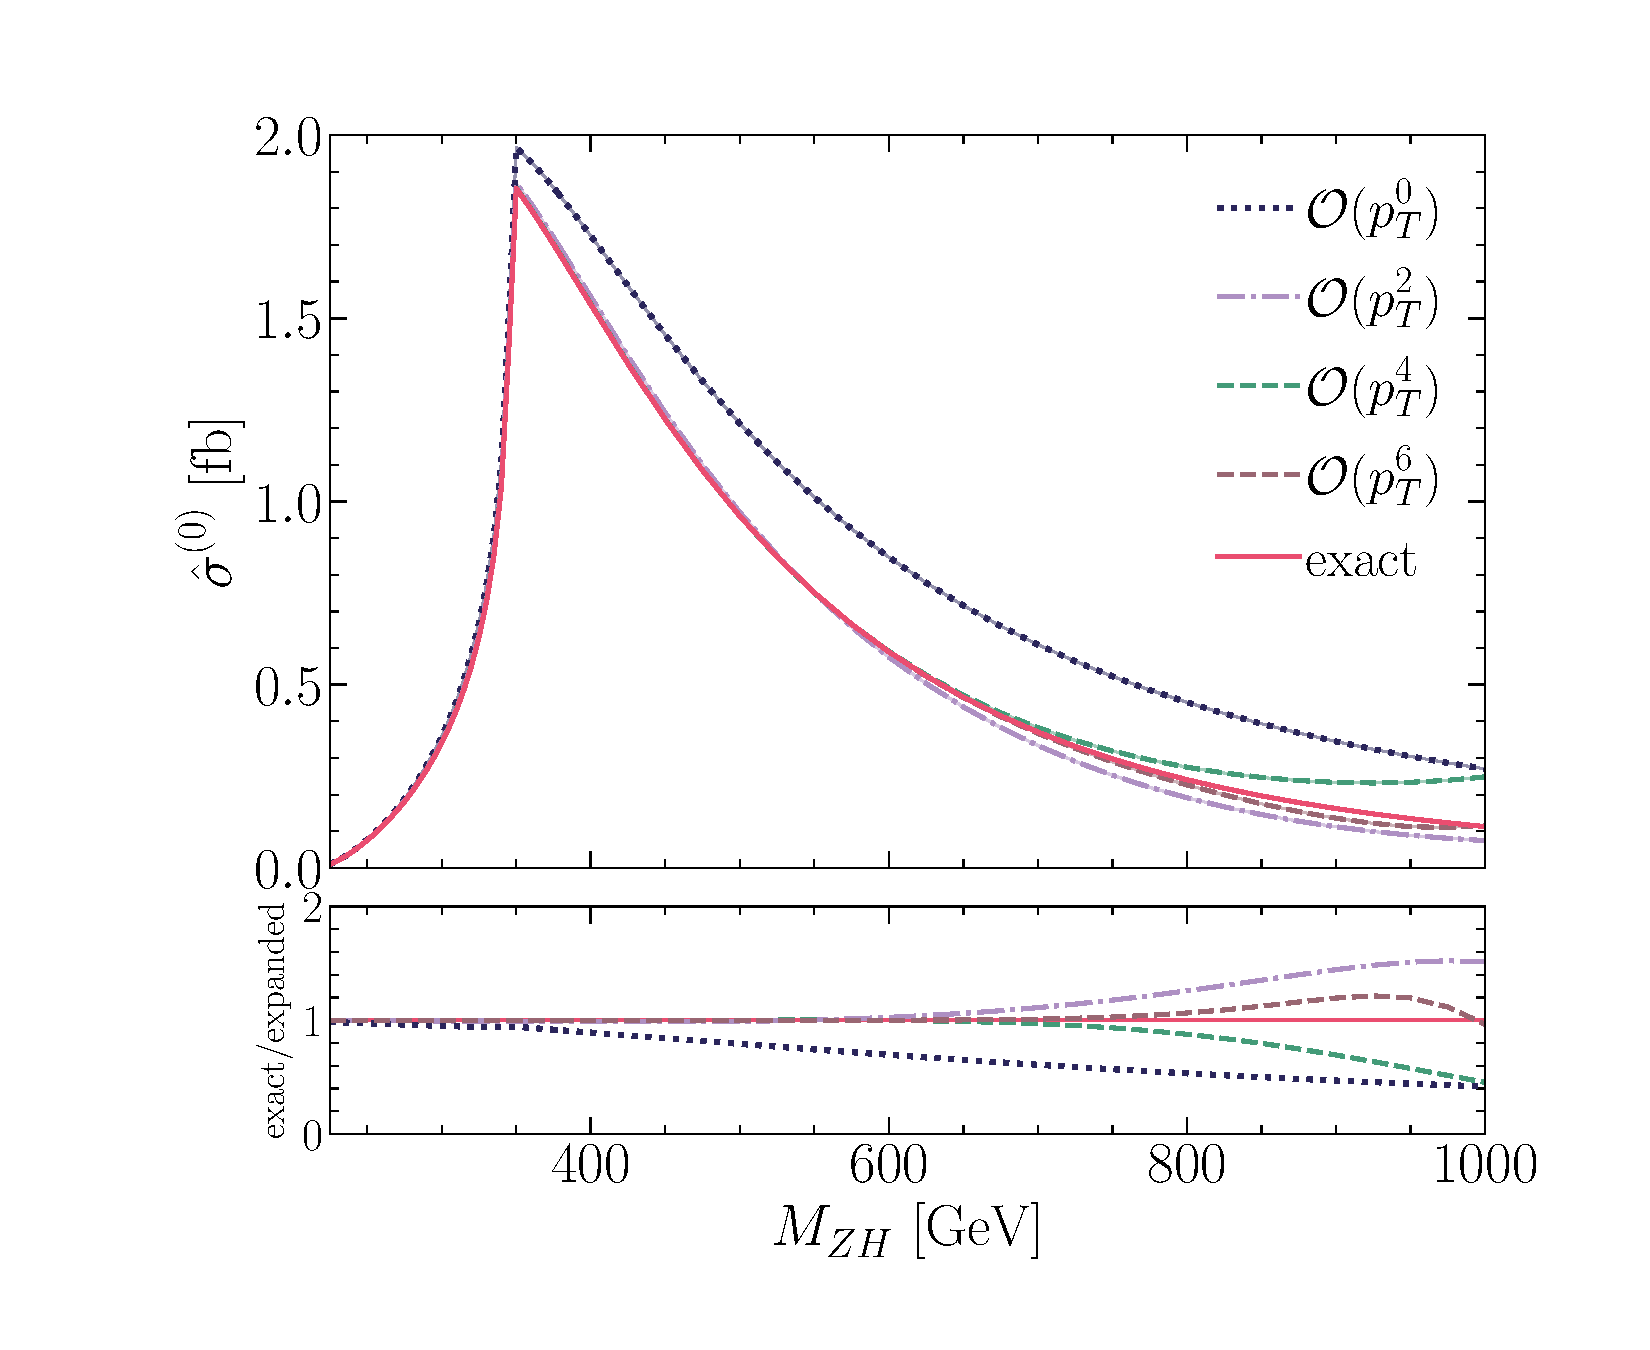
\includegraphics[width=0.8\linewidth]{./figures/LO_ptexp_ratio_1000.pdf}
	\caption{The Born partonic cross-section
		as a function of the invariant mass $M_{Zh}$.
		The exact (red line) is plotted together with results at
		different orders in the $\pt$-expansion (dashed lines). In the bottom part,
		the ratio of the full result over the $\pt$-expanded one at
		various orders is shown. This plot has been already published in~\cite{Alasfar:2021ppe}}
	\label{fig:LO}
\end{figure}
From the ratio plotted in the lower panel of ~\autoref{fig:LO} , we observe that the~$\mathcal{O}(\pt^0)$ expansion is in good agreement with the exact result  when $M_{Zh}\lesssim 2\mt$. Inclusion of higher order terms up tp~$\mathcal{O}(\pt^6)$ extended the validity of the expansion to reach  $M_{Zh}\lesssim 750\gev$. This is the similar behaviour seen in ~\cite{Bonciani:2018omm} for Higgs pair.  Therefore, one would expect the $\pt$-expanded two-loop virtual correction to be an accurate approximation with the exact (numerical) result for the region of the invariant mass of  $M_{Zh}\sim 700-750\gev$. 
Similar conclusions can be seen more explicitly in~\autoref{tab:partonic}, where it is shown that the partonic cross-section
at $\mathcal{O}(\pt^4)$ agrees with the full result for
$M_{ZH} \lesssim 600 \gev$  on the permille level 
and the agreement further improves when $\mathcal{O}(\pt^6)$ terms are included.
\begin{table}
	\renewcommand{\arraystretch}{1.2}
	\centering
	\begin{tabular}{| c| c | c | c| c| c|} \hline
		\rowcolor{lightgray}  $M_{Zh}$ [GeV]  & $\mathcal{O}(\pt^0)$ & $\mathcal{O}(\pt^2)$ & $\mathcal{O}(\pt^4)$ & $\mathcal{O}(\pt^6)$ & full \\ \hline 
		\cellcolor{lightgray} 300 & 0.3547 & 0.3393 &  0.3373 &0.3371& 0.3371 \\
		\cellcolor{lightgray} 350 & 1.9385 & 1.8413& 1.8292 &1.8279& 1.8278 \\
		\cellcolor{lightgray} 400 & 1.6990 & 1.5347 & 1.5161 &1.5143& 1.5142 \\
		\cellcolor{lightgray} 600 & 0.8328 & 0.5653 & 0.5804 &0.5792&  0.5794 \\ 
		\cellcolor{lightgray} 750 & 0.5129 & 0.2482 & 0.3129 & 0.2841 &  0.2919 \\ \hline
	\end{tabular}
	\caption{The partonic cross section $\hat{\sigma}^{(0)}$ at
		various orders in $\pt$ and the full computation for several values of $M_{Zh}$, This table has been already published in~\cite{Alasfar:2021ppe}. \label{tab:partonic}}
\end{table}
%%%%%%%
\section{ NLO calculation }
\label{sec:quattro}
The virtual two-loop corrections to~$ gg\to Zh$ are shown in~\autoref{fig:dianlo}, which involve corrections to the triangle topology in (a) and (b). The corrections to the box topology in (c) and a new topology , dented by double triangle in (d). Both two-loop corrections to the triangles, and the double triangle diagrams can be computed exactly analytically. However, the two-loop box diagrams contain master-integrals~(MI's) that have no analytic solutions, so far. The two-loop box diagrams will be computed in the $\pt$-expansion.
\begin{figure}[htpb!]
	\begin{center}
		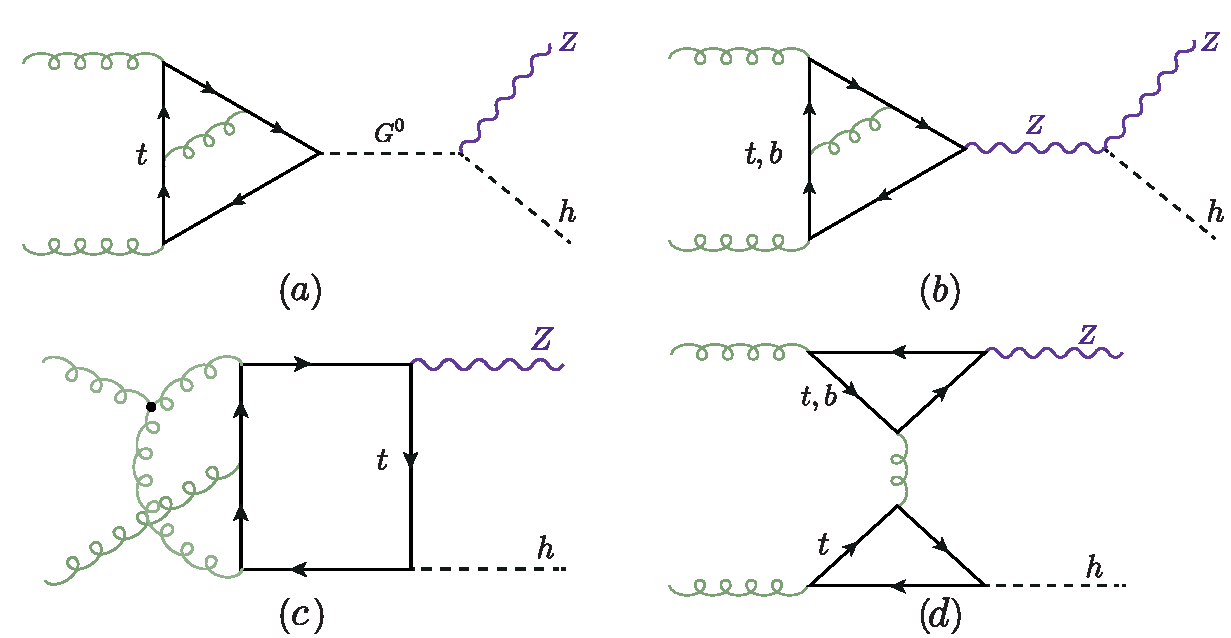
\includegraphics[width=12cm]{./figures/Feynman_NL0}
		\caption{Feynman diagrams types for the virtual NLO corrections to the $gg \to Zh$ process. }
		\label{fig:dianlo}
	\end{center}
\end{figure}
\subsection{Renormalisation}
\label{subsec:ren}
The two-loop corrections to the triangle and box diagrams contain both UV and IR divergences. The first emerges from UV divergent sub-diagrams, such as top mass renormalisation and QCD vertex correction. While the lR divergences come from massless loops. In order to remove these divergences, one introduces adequate counter-terms.  On the other hand, the double triangle is both UV and IR finite.
\par  We start by the gluon wavefunction renormalisation of the incoming gluons  (external legs) such that the amplitude is renormalised by $ Z_A^{1/2}$ for each gluon.
\begin{equation}
	Z_A= 1+\as \frac{2}{3\epsilon} \left( \frac{\mu_R^2}{m_t^2} \right) ^\epsilon.
\end{equation}
 The on-shell scheme for the top mass renormalisation has been used, in which the bare mass is replaced by the renormalised one~$ m_0 = Z_m m$  in the propagators this gives the $\MSbar$ renormalised mass. 
 %This can be done with multiplying $ \delta Z_m$ with the derivative of the one-loop form-factor with respect to the  mass., here $Z_m$ is given by
\begin{equation}
	Z_m = 1+ C_F \frac{3}{\epsilon}.
\end{equation}
In order to convert the mass definition to the on-shell scheme we add the finite renormalisation term
\begin{equation}
	Z^{OS}_m = 1- 2 C_F,
\end{equation}
here $C_F=(N_c^2-1)/2N_c$ is one of the two Casimir invariants of QCD along with~$ C_A=N_c$. 
The $q \bar q g$ vertex correction involves a renormalisation of the strong couplings constant $ \alpha_s$ which is done via replacing the bare constant $\alpha_s^0$ with the renormalised one, hence it becomes  $ \alpha^0_s = \frac{\mu_R^{2\epsilon}}{S_\epsilon}  \Zas \alpha_s$, where
\begin{equation}
	\Zas = 1- \frac{\alpha_s}{4 \pi} \, \frac{1}{ \epsilon}\,  \left( \beta_0-\frac{2}{3} \right) \left(\frac{\mu_R^2}{m_t^2} \right) ^\epsilon,
\end{equation}
and the constant $ \beta_0 = \frac{11}{3} C_A -\frac{2}{3}N_f$, where $N_f$ is the number of ``active'' flavours. The 5-flavour scheme $N_f=5$ is adopted here. 
\par The loop integrals were evaluated via dimensional regularisation in $d= 4-2\epsilon$ dimensions. Which requires some caution when $\gamma_5$ is present in the amplitude. We let $\gamma_5$ naively anti-commute with all $d$-dimensional $\gamma_\mu$'s and then correct that with the finite renormalisation constant known as \textbf{ Larin counter-term}~\cite{Larin:1993tq}
\begin{equation}
	Z_5 = 1- 2\, C_F.
\end{equation}
The renormalised amplitude is written as
\begin{equation}
	\mathcal M  (\alpha_s, m, \mu_R) = Z_A \mathcal M( \alpha_s^0, m^0).
\end{equation}
Putting all the above substitutions together, we get the renormalised  two-loop form-factor:
\begin{align}
	( \mathcal A ^{(1)})^R &= 	\mathcal A ^{(1)} -	\mathcal A_{UV} ^{(0)}- 	\mathcal A_{UV, m} ^{(0)} + \mathcal A_{\text{Larin}} ^{(0)}   \\
	\mathcal A_{UV} ^{(0)} &= \asr\,\frac{\beta_0}{\epsilon} \left( \frac{\mu_R^2}{\hat s} \right) ^{ -\epsilon} 	\mathcal A ^{(0)}.  \nonumber \\
	\mathcal A_{UV, m} ^{(0)} &= \asr \, \left( \frac{3}{\epsilon} -2\right) C_F \left( \frac{\mu_R^2}{\hat s} \right) ^{ -\epsilon} m^0 \partial_m \mathcal A^{(0)} . \nonumber \\
	\\
	\mathcal	A_{\text{Larin}} ^{(0)}  &= - \asr \, C_F  \mathcal A ^{(0)} .\nonumber
\end{align}
The following IR-counter-term is used in order to cancel the IR divergences.
\begin{equation}
	\mathcal A_{IR} ^{(0)}  = \frac{e^{\gamma_E \epsilon}}{\Gamma(1-\epsilon)} \, \asr \left( \frac{\beta_0}{\epsilon} + \frac{ C_A}{\epsilon^2} \right)  \, \left(  \frac{\mu_R^2}{\hat s}\right) ^{2\epsilon} \mathcal A ^{(0)}
\end{equation}
The one-loop form-factors, need to be expanded up to order $ \mathcal O(\epsilon^2) $, for the UV and IR counter-terms.
\subsection{Calculation of the exact virtual corrections}
The two-loop calculations of the triangle digrams involves the diagrams of with virtual $Z^*$ and $G^0$, depending on the gauge of choice. Observations found in ref.\cite{Altenkamp:2012sx} shows that due to Landau-Yang theorem  in the Landau gauge the diagrams with the  $Z^*$ exchange vanishes. Therefore, the part of the top triangle diagrams  can be obtained from the decay amplitude of a pseudoscalar boson into two gluons which is  known in the literature in the full mass dependence up to NLO terms \cite{Spira:1995rr,Aglietti:2006tp}. On the contrary, in the unitary gauge, the NLO calculation needs to be done with the $Z^*$ exchange diagrams only.  The calculations result in apparently different Lorentz structures, that are linked via the Schouten identity 
\begin{equation}
q^\alpha \epsilon^{\beta \gamma \delta  \phi} + q^\beta \epsilon^{\gamma \delta  \phi \alpha}+ q^\gamma \epsilon^{ \delta  \phi \alpha \beta} +q^\gamma \epsilon^{ \delta  \phi \alpha \beta} + q^\delta \epsilon^{   \phi \alpha \beta \gamma } +  q^\phi \epsilon^{ \alpha \beta \gamma \delta } =0 
\end{equation}
A cross-check has been preformed in order to ensure that the NLO calculation introduces no new Lorentz structures, and gives the same result in a general $ R_\xi$ gauge as the results in~\cite{Spira:1995rr,Aglietti:2006tp}. The two-loop calculation has been carried out in~ $ R_\xi$ gauge. The amplitudes have been automatically generated by \texttt{FeynArts} \cite{Hahn:2000kx} and
contracted with the projectors as defined in \autoref{app:uno}
using \texttt{FeynCalc }\cite{Mertig:1990an,Shtabovenko:2016sxi} and \texttt{Package X}~\cite{Patel:2016fam} and in-house
Mathematica routines. The two-loop integrals were reduced to a set of master integrals~MI, illustrated graphically in~\autoref{fig:trimis} using \texttt{Kira}~\cite{Maierhofer:2017gsa}.
\begin{figure}[htpb!]
	\begin{center}
		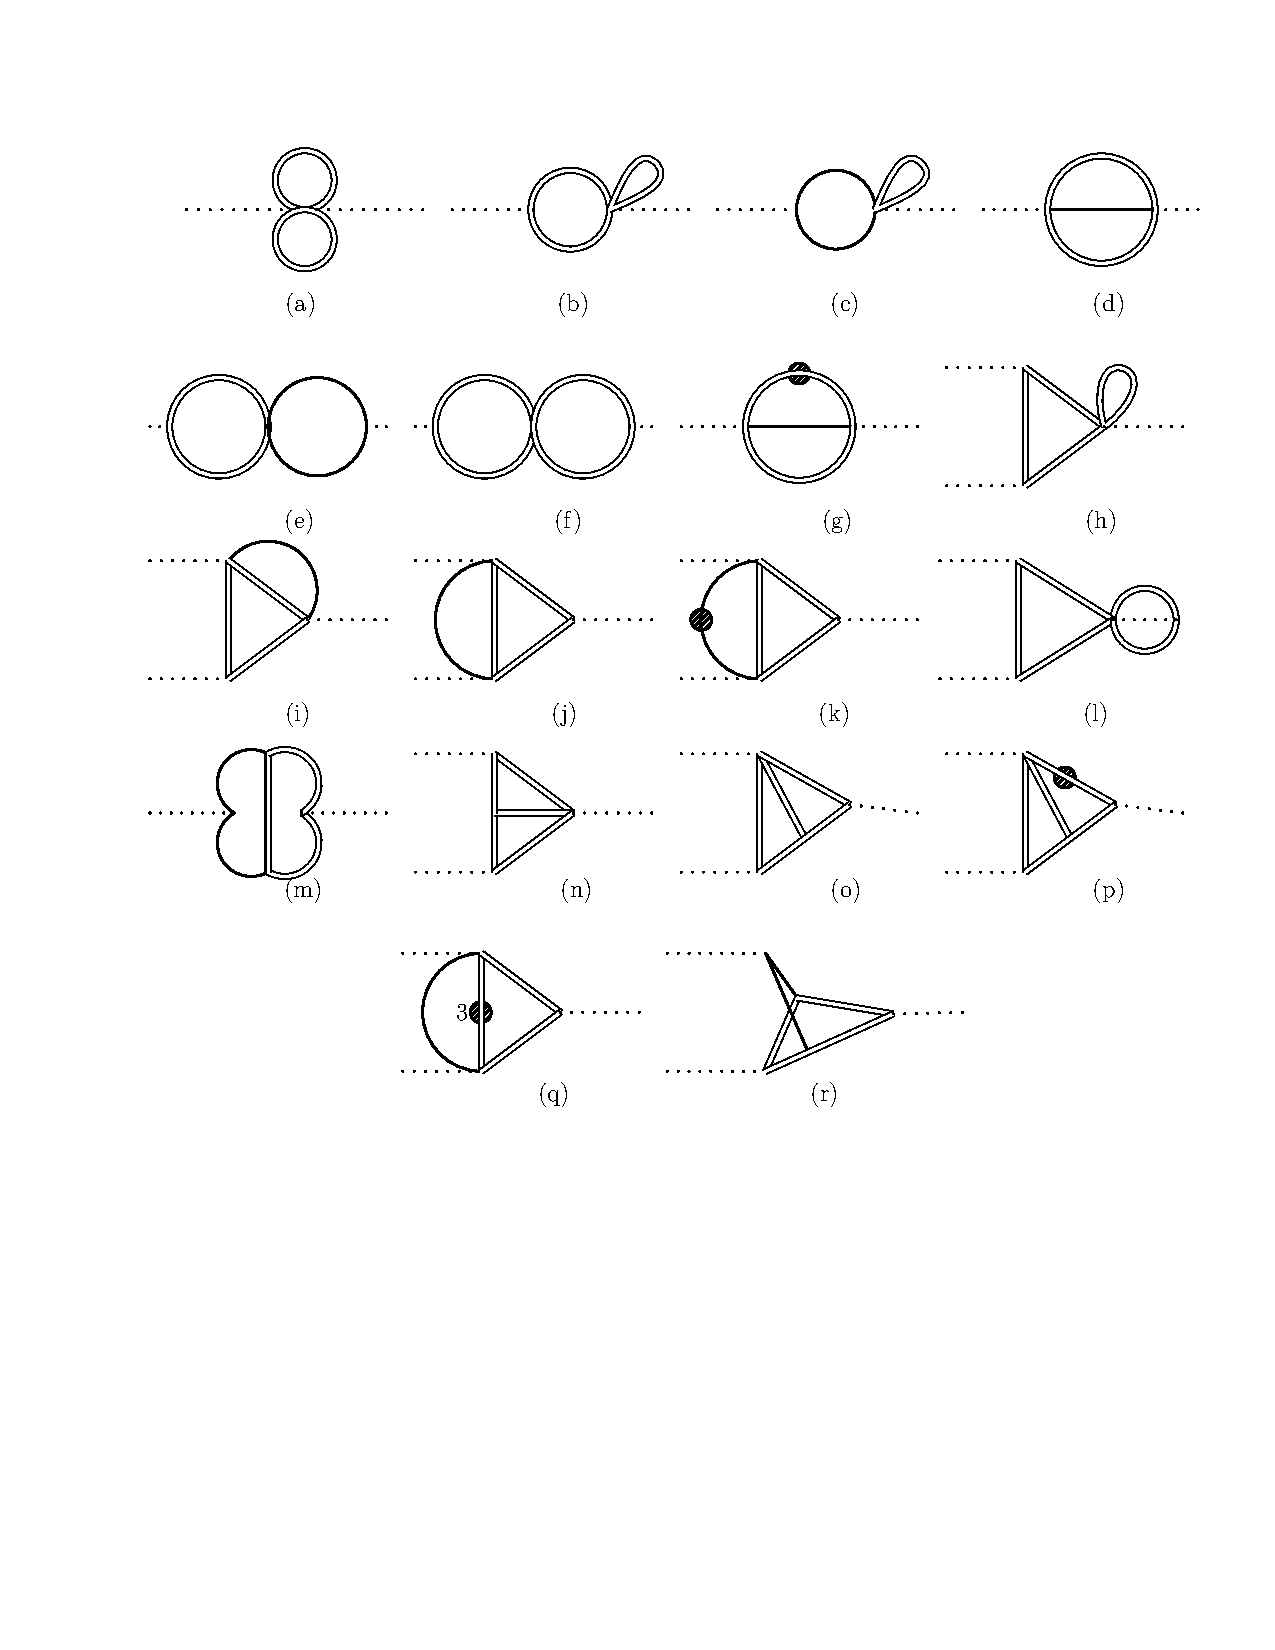
\includegraphics[width=12cm]{./figures/MI}
		\caption{ The list of two-loop  master integrals (MI's) resulting from the reduction of the two-loop triangle corrections, and the product of one-loop MI's appearing in this list also appear in the calculation of the double-triangle diagrams. A single line denotes a massless propagator, while a double line denotes a massive one. The dot denotes a squared propagator, unless the number of the exponent is indicated, here only $3$ appears in diagram (q). }
		\label{fig:trimis}
	\end{center}
\end{figure}
These MI's  are either products of one-loop functions (a)-(c), (e),(f),(h) and (l) or can be found in the literature~\cite{Bonciani:2003hc,Aglietti:2006tp}. Their implementation in our calculation has been validated numerically using \texttt{SecDec}~\cite{Borowka:2013cma,Borowka:2015mxa}.  
The virtual correction for the triangle diagrams can be separated according to their colour factors into
\begin{equation}
	\mathcal A ^{(1)}   = C_F \mathcal A_{CF} ^{(1)}  + C_A \mathcal A_{CA} ^{(1)},
\end{equation}
The $C_A$ part contains a double pole $ \mathcal O( 1/\epsilon^2) $  and a single pole $ \mathcal O( 1/\epsilon) $, both  coming from the IR divergence. Whilst the $C_F$ part contains a UV divergent pole that needs to be cured via mass renormalisation. The poles do not have a dependence on the renormalisation scale $ \mu_R$. However, there is a dependence on that scale in the finite part, as well.  No new Lorentz structures appeared, and the final result in $R_\xi$ matched the one found in~\cite{Spira:1995rr,Aglietti:2006tp} for the Landau gauge. The explicit results are shown in~\autoref{app:due}
%
\par  The calculation of the double triangle diagrams (d) of~\autoref{fig:dianlo} is fairly straightforward, all of the 
 integrals can be rewritten in terms of products of one-loop functions. All of the Lorentz structures appear in the double triangle except for $\mathcal{P}_6$, analogous to the triangle case. The explicit forms of form-factors corresponding to these structures are presented in~\autoref{app:due}. Although we write the amplitude using a different
tensorial structure with respect to ref.\cite{Davies:2020drs} we have checked,
using the relations between the two tensorial structures reported in 
\autoref{app:uno}, that our result is in agreement with the one presented
in ref.\cite{Hasselhuhn:2016rqt}.
\subsection{Calculation of the $\pt$-expanded virtual corrections}
%%%
\par The two-loop triangle diagrams can also be interpreted as an expansion in $\pt$, but this expansion terminates at~${\cal O}(\pt^2)$, rather being an infinite series. Hence, in this section we concentrate on the two-loop box diagrams $\pt$-expansion~\footnote{The calculation of the box diagrams has been done mainly by my collaborators, the co-authors of~\cite{Alasfar:2021ppe}}.\\
%%%%
Similar to the two-loop triangle diagrams, the box diagrams amplitudes were generated projected through the same pipeline. After the contraction of the epsilon tensors the diagrams were expanded as
described in \autoref{sec:ptexp}, keeping only ${\cal O}(\pt^4)$ terms. They were reduced to MI's
using \texttt{FIRE} \cite{Smirnov:2014hma} and \texttt{LiteRed} \cite{Lee:2013mka}. The
resulting MI's were identical to the one for Higgs pair
production \cite{Bonciani:2018omm}. Nearly all of them are expressed
in terms of generalised harmonic polylogarithms with the exception of
two elliptic integrals \cite{vonManteuffel:2017hms, Bonciani:2018uvv}. The renormalisation and IR pole subtraction procedure was carried out like prescribed~\autoref{subsec:ren}.\\
As a control, the two-loop box diagrams were also computed in the LME up to  $\mathcal{O}(1/\mt^6)$. Since this expansion should be included within the $\pt$-expansion. We have retained the LME analytic expression by further expanding the $\pt$-expanded amplitude in small ~$\hat{s}/\mt^2$. Providing an additional cross-check for the validity of the $\pt$-expansion.
%%%%%
\section{Results and conclusions} \label{sec:hzres}
The virtual corrections to the gluon fusion $Zh$ production have been implemented in a  \texttt{FORTRAN} code using  \texttt{handyG} \cite{Naterop:2019xaf}, for the evaluation of generalised harmonic polylogarithms, \texttt{Chaplin}~\cite{Buehler:2011ev} for the harmonic polylogarithms appearing in the triangle two-loop functions  while 
the elliptic integrals are evaluated using the routines of
ref.\cite{Bonciani:2018uvv}. Since the result is analytic, the code is significantly faster than the numerical evaluation of the two-loop amplitude~\cite{Chen:2020gae}, with evalution time of ca. 0.5 min per one phase space point on a personal laptop.\\
In order to facilitate the comparison of our results with the ones
presented in the literature, we define the finite part of the virtual corrections
as in
ref.\cite{Davies:2020drs}\footnote{The definition of the matrix elements here
	differs by a factor of
	$\frac{1}{\hat{s}}$ from ref.\cite{Davies:2020drs}, \textit{cf}. also
	 \autoref{app:uno}.}
\begin{equation}
	\begin{split}
		\mathcal{V}_{fin}&=\frac{G_F^2 m_Z^2}{16}\left(\frac{\alpha_s}{\pi}\right)^2
		\left[ \sum_{i} \left|\mathcal{A}_i^{(0)} \right|^2\frac{C_A}{2}\left(\pi^2-
		\log^2\left(\frac{\mu_R^2}{\hat{s}}\right)\right)\right. \\
		& \left. +2\sum_i\text{Re}\left[\mathcal{A}_i^{(0)}\left(\mathcal{A}_i^{(1)}\right)^*\right]\right]\,
		\label{eq:vfin}
	\end{split}
\end{equation}
and in the numerical evaluation of eq.(\ref{eq:vfin}) we fixed
$\mu_R= \sqrt{\hat{s}}$.
Triangle and LME box toopologies were validated against the results of refs.\cite{Hasselhuhn:2016rqt,Davies:2020drs} finding perfect
agreement at the form-factor level, i,.e.$\mathcal{A}_i^{(1)}$. 

The virtual part of the partonic cross-section
from the finite part of the virtual corrections in eq.\eqref{eq:vfin} is defined  by
\begin{equation}
	\Delta \hat{\sigma}_{virt}=
	\int_{\hat{t}^-}^{\hat{t}^+} d\hat{t}
	\frac{\alpha_s}{16\pi^2}\frac{1}{\hat{s}^2}\mathcal{V}_{fin}\,
	\label{eq:deltasigma}
\end{equation}
This function is used to confront $\pt$-expanded results. Starting with low $M_{Zh}$ we have compared the $\pt$-expanded with the LME 	$\mathcal{V}_{fin}$, finding a  good numerical agreement.
It is important to note that, at the same order in the expansion, 
the $\pt$-expanded terms are more accurate than
the LME ones, although computationally more demanding.  Additional checks have been done using the numerical evaluation of the NLO amplitude by \cite{Chen:2020gae}, where they have evaluated the exact two-loop MI's using \texttt{pySecDec}
\cite{Borowka:2017idc,Borowka:2018goh}.  \autoref{tab:comparison} shows a comparison between our $\pt$-expanded~$\mathcal{V}_{fin} 4/(\as^2 \alpha^2)$ versus the exact numerical result of ~\cite{Chen:2020gae} for several phase space points. 
As can be seen from the table the relative difference 
between the two results is less than half a permille.
\begin{table}
	\renewcommand{\arraystretch}{1.2}
	\centering
	\begin{tabular}{| c| c | c | c| } \hline
		\rowcolor{lightgray}  $\hat{s}/m_t^2$ & $\hat{t}/m_t^2$ &  ref.\cite{Chen:2020gae} & $\mathcal{O}(\pt^6)$  \\ \hline 
		\cellcolor{lightgray} 1.707133657190554 & \cellcolor{lightgray} -0.441203767016323 & 35.429092(6) & 35.430479 \\
		\cellcolor{lightgray} 3.876056604162662 & \cellcolor{lightgray} -1.616287256345735 & 4339.045(1) & 4340.754 \\
		\cellcolor{lightgray} 4.130574250302561 & \cellcolor{lightgray} -1.750372271104745 & 6912.361(3) & 6915.797 \\
		\cellcolor{lightgray} 4.130574250302561 & \cellcolor{lightgray} -2.595461551488002 & 6981.09(2) & 6984.20  \\ \hline
	\end{tabular}
	\caption{Comparison of $\mathcal{V}_{fin} 4/(\alpha_s^2 \alpha^2)$ with the numerical results of ref.\cite{Chen:2020gae}. This plot has been already published in~\cite{Alasfar:2021ppe}. \label{tab:comparison}}
\end{table}
\begin{figure}[th]
	\centering
	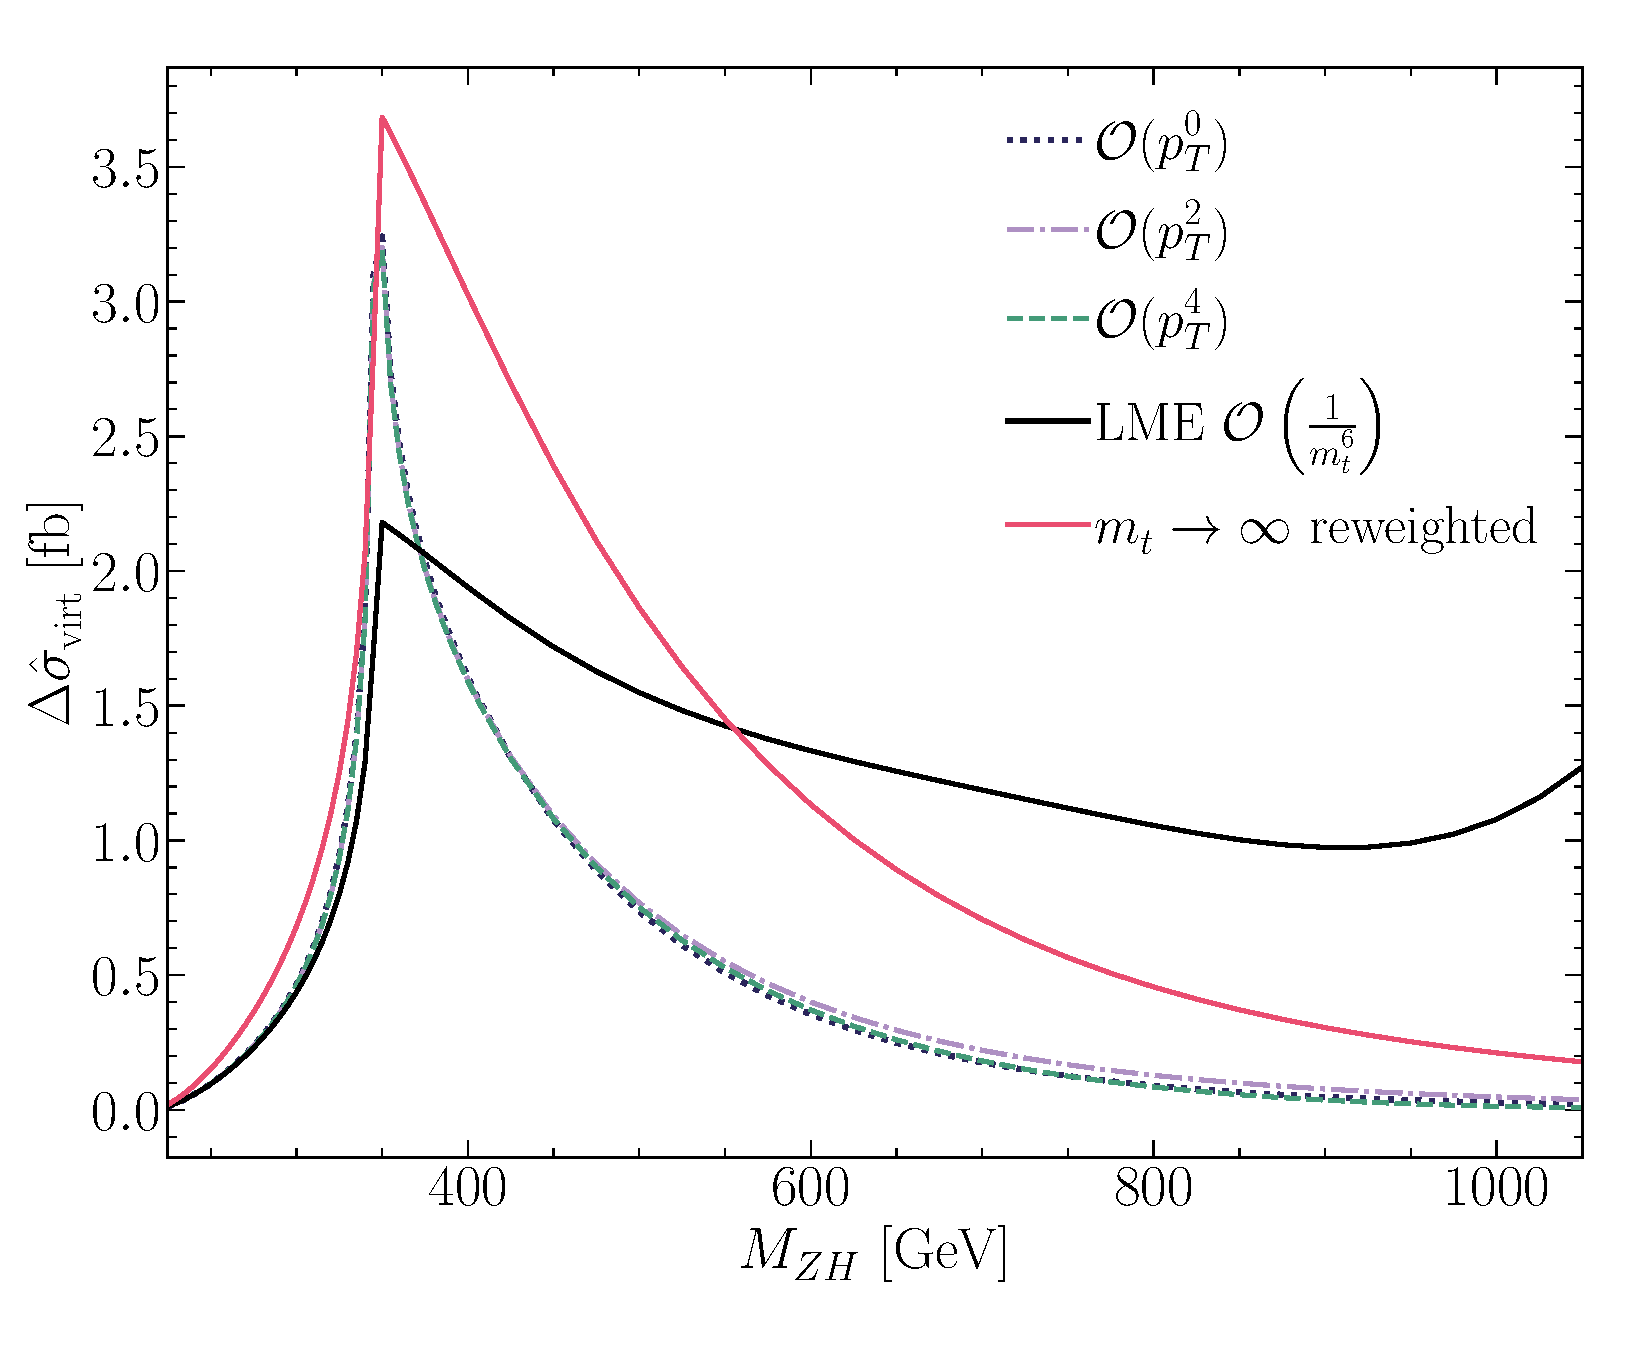
\includegraphics[width=0.7\textwidth]{./figures/sigma_part_virt_LMEreweighted.pdf}
	\caption{$\Delta \hat{\sigma}_{virt}$ defined by eq.\eqref{eq:deltasigma}, shown as a function of $M_{ZH}$. The various orders of the $\pt$-expansion are plotted as dashed lines, while the black and red continuous lines stand for the LME and  reweighted $m_t \rightarrow \infty$ results, respectively.This plot has been already published in~\cite{Alasfar:2021ppe}.}
	\label{fig:deltasigma}
\end{figure}
%%%%%%%%%%

In \autoref{fig:deltasigma}, the dashed lines show
 the different orders of the expansion. 
For all parts of the matrix elements the best results
available, i.e.~both $\mathcal{A}^{(0)}$ were used and the double-triangle
contribution are evaluated exactly, while for
$\mathcal{A}^{(1)}$ we use the various orders in the $\pt$-expansion.
For comparison, the results are shown were
$\mathcal{A}^{(1)}$ is replaced by the one computed in LME up to
$\mathcal{O}(1/m_t^6)$ (full black line), which as mentioned before is valid
up to $M_{ZhH}< 2 \mt$. We observe that within the validity of the LME our
results agree well with it.
Furthermore, the results in the infinite top
mass limit reweighted by the full amplitudes squared can be seen as the full red line in the plot, corresponding to the
approach of ref.\cite{Altenkamp:2012sx}, keeping though the double triangle
contribution in full top mass dependence. 
Differently from the LME line, the $\mt \to \infty$ reweighted one
shows a behaviour, for  $M_{Zh} \gtrsim 400\gev$, similar to the behaviour of
the $\pt$ lines. Still,   the difference
between the reweighted result and the $\pt$-expanded ones is  significant.
The $\pt$-expanded results show
very good convergence.  The zero order in our expansion agrees
extremely well with the higher orders in the expansion, and all the
three results are very close up to $M_{Zh} \sim 500\gev$.
%%%%%%%%%%%%%%%%%%%%%%%%%%%%%%%
\par  The calculation of the virtual two-loop corrections to the $gg \to Zh$ is done using exact results for the triangle and double-triangle topologies, and in the $\pt$-expansion for the box one.  The result of the calculation showed that we get the exact same MI's that was found for Higgs pair production \cite{Bonciani:2018omm} , mostly these MI's are expressed in terms of generalised harmonic polylogarithms with the
exception of two elliptic integrals. Using the LO calculation, we have shown the validity of the $\pt$-expansion covering the invariant mass interval  $M_{Zh}\lesssim 750\text{ GeV}$ which covers $\sim 98\%$ of the total phase space for~$13-14$ TeV energies.\\
The $\pt$-expansion agrees with per mill level with the numerical results found in ~\cite{Chen:2020gae}. However, it allows for fast computation of the amplitude with circa one second per phase space point using a modern laptop with mid-range specifications. Additionally. the integration over the $\hat{t}$ variable
in eq.(\ref{eq:deltasigma}) converges very well.  The flexibility of our analytic
results, an application to beyond-the-Standard Model is certainly
possible.\\ 
Finally, it should be noted that this calculation complements
nicely the results obtained in ref.\cite{Davies:2020drs} using a high-energy
expansion, that according to the authors provides precise results for
$\pt \gtrsim 200\gev$. The merging of the two analyses is going to provide
a result that covers the whole phase space, can be easily implemented into a
Monte Carlo code using v which is currently a work in progress in \la{Cite the new paper here-later}